\vspace{-10pt}
\section{Preemption Point Placement Algorithm}\label{sec:implementation}

Our approach employs the results of schedulability analysis and the aforementioned WCET + CRPD calculation with the maximum allowable non-preemption region parameter \begin{math}Q_{i}\end{math} computed for each task \begin{math}\tau_{i}\end{math}.  The objective is to select a subset of preemption points that minimizes each tasks WCET + CRPD parameter \begin{math}C_{i}\end{math}. The selection of optimal preemption points is subject to the constraint that no non-preemptive region in task \begin{math}\tau_{i}\end{math} exceeds the maximum allowable non-preemption region parameter \begin{math}Q_{i}\end{math}:
\begin{equation}\label{eqn:pp-constraint}
   \Psi_{i}(\rho_{i}) =
\left\{
\begin{array}{lr}
    \textrm{True, }&\textrm{if } q_{i}^{m}(\rho_{i}) \leq Q_{i} \textrm{ for } m \in [1,|\rho_{i}|-1] \\
    \textrm{False, }&\textrm{otherwise}
\end{array}
\right\}~
\end{equation}

\noindent
where \begin{math}q_{i}^{m}(\rho_{i})\end{math} represents the \begin{math}m^{th}\end{math} non-preemptive-region (NPR) time for task \begin{math}\tau_{i}\end{math}:
\begin{equation}\label{eqn:mthnpr-time}
   q_{i}^{m}(\rho_{i}) = \Big[\xi_{i}(\rho_{i}^{m},\rho_{i}^{m+1}) + \sum_{n=\rho_{i}^{m}}^{\rho_{i}^{m+1}}b_{i}^{n}\Big]
\end{equation}

\noindent
In accordance with the recursive nature of equation (\ref{eqn:bbkwcet-cost}) we propose an O(N!) recursive algorithm shown in Algorithm~\ref{alg:recursive-optimal-ppp} for computing the optimal preemption points.  While the recursive formulation is clearly inefficient, it is helpful in developing an understanding of how the algorithm works.  Starting with the first basic block and for each successive basic block \begin{math}\delta_{i}^{m}, m \in [1,N_{i}]\end{math}, the overall WCET cost is computed for two cases: 1) \begin{math}\delta_{i}^{m} \in \rho_{i}\end{math}, and 2) \begin{math}\delta_{i}^{m} \not\in \rho_{i}\end{math}.  At each step of the algorithm the set \begin{math}\rho_{i}\end{math} must conform to the constraint of equation (\ref{eqn:pp-constraint}).  Once basic block \begin{math}\delta_{i}^{N_{i}}\end{math} has been examined, the set of selected preemption points is given by \begin{math}\rho_{i} = \rho_{i}^{(N_{i})}\end{math}.  The WCET cost with basic block \begin{math}\delta_{i}^{m}\end{math} included in the set of potential preemption points is given by:
\begin{equation}\label{eqn:pcost-bb}
p_{COST}(\delta_{i}^{m})\ =\ B_{i}^{0,m}(\rho_{i}) + B_{i}^{m,N_{i}}(\rho_{i})
\end{equation}

The WCET cost with basic block \begin{math}\delta_{i}^{m}\end{math} excluded from the set of potential preemption points is given by:
\begin{equation}\label{eqn:npcost-bb}
n_{COST}(\delta_{i}^{m})\ =\ B_{i}^{0,m-1}(\rho_{i}) + b_{i}^{m} + B_{i}^{m+1,N_{i}}(\rho_{i})
\end{equation}

{\fontsize{10}{10}\selectfont
\begin{algorithm}
\caption{Recursive Optimal Preemption Point Placement}
\label{alg:recursive-optimal-ppp}
\begin{algorithmic}[0]
\small
\State \textbf{\underline{Step 0:}}
%\\
\State {$\ \ \rho_{i}^{(0)}\ \gets\ \{\delta_{i}^{0},\delta_{i}^{N_{i}}\}$};
\State {$\ \ \textbf{if}\ \Psi_{i}^{N_{i}}(\{\delta_{i}^{0},\delta_{i}^{1},\delta_{i}^{2}, ..., \delta_{i}^{N_{i}}\}) = False$\ \textbf{then}}
\State {$\ \ \ \ \ \ \textbf{return}\ \textbf{INFEASIBLE;}$}
\State {$\ \ \textbf{end if}$}
\\
%\State \textbf{\underline{Step 1:}}
%\begin{equation*}
%\rho^{(1)}\ \gets\
%\left\{
%\begin{array}{l}
%    \rho^{(0)}, if\ n_{COST}(\delta_{i}^{1}) < p_{COST}(\delta_{i}^{1})\ \&\ \ \ \ \ \ \ \ \ \ \ \\
%    \ \ \ \ \ \ \ \ \ \ \Psi_{i}^{1}(\rho^{(0)}) = True\\
%    \rho^{(0)}\ \cup\ \delta_{i}^{1},\ otherwise
%\end{array}
%\right\}~
%\end{equation*}
%\State \textbf{\underline{Step 2:}}
%\begin{equation*}
%\rho^{(2)}\ \gets\
%\left\{
%\begin{array}{l}
%    \rho^{(1)}, if\ n_{COST}(\delta_{i}^{2}) < p_{COST}(\delta_{i}^{2})\ \&\ \ \ \ \ \ \ \ \ \ \ \\
%    \ \ \ \ \ \ \ \ \ \ \Psi_{i}^{2}(\rho^{(1)}) = True\\
%    \rho^{(1)}\ \cup\ \delta_{i}^{2},\ otherwise
%\end{array}
%\right\}~
%\end{equation*}
%\ldots
\State \textbf{\underline{Steps m = 1,\ \ldots,\ $N_{i}$:}}
\begin{equation*}
\rho_{i}^{(m)}\ \gets\
\left\{
\begin{array}{l}
    \rho_{i}^{(m-1)}, if\ n_{COST}(\delta_{i}^{m}) < p_{COST}(\delta_{i}^{m})\ \&\ \ \ \ \\
    \ \ \ \ \ \ \ \ \ \ \ \ \ \Psi_{i}^{m}(\rho_{i}^{(m-1)}) = True\\
    \rho_{i}^{(m-1)}\ \cup\ \delta_{i}^{m},\ otherwise
\end{array}
\right\}~
\end{equation*}
%\ldots
%\State \textbf{\underline{Step $N_{i}$:}}
%\begin{equation*}
%\rho^{(N_{i})}\ \gets\
%\left\{
%\begin{array}{l}
%    \rho^{(N_{i}-1)}, if\ n_{COST}(\delta_{i}^{N_{i}}) < p_{COST}(\delta_{i}^{N_{i}})\ \&\\
%    \ \ \ \ \ \ \ \ \ \ \ \ \ \ \Psi_{i}^{N_{i}}(\rho^{(N_{i}-1)}) = True\\
%    \rho^{(N_{i}-1)}\ \cup\ \delta_{i}^{N_{i}},\ otherwise
%\end{array}
%\right\}~
%\end{equation*}
\normalsize
\end{algorithmic}
\end{algorithm}
}
\noindent
The recursive formulation gives a preliminary algorithm description, however, it is computationally intractable.  We now propose an \begin{math}O(cN^{2})\end{math} dynamic programming algorithm for computing the optimal preemption points.  In support of our dynamic programming algorithm, we propose the following theorem claiming optimal substructure of our solution formulation in terms of the WCET + CRPD cost $B_{i}$.

\begin{theorem}
\label{thm:optimal-substructure-cost}
The WCET + CRPD cost variable $B_{i}$ utilized in our solution exhibits optimal substructure.
\end{theorem}

\noindent
We now prove the optimal substructure property of the WCET + CRPD cost $B_{i}$.
\newline
\noindent
\begin{proof}
Let $B_{i}^{j,k}(\rho_{i})$ with its corresponding selected preemption points denoted by $\rho_{i}^{j,k}$ be the optimal limited preemption execution cost solution from basic block $j$ to basic block $k$, and assume the optimal cost solution contains the basic block identified by $m$. Furthermore, let $B_{i}^{j,m}(\rho_{i})$ with selected preemption points denoted by $\rho_{i}^{j,m}$ and $B_{i}^{m+1,k}(\rho_{i})$ with selected preemption points denoted by $\rho_{i}^{m+1,k}$ be the optimal limited preemption execution cost from $j$ to $m$ and from $m+1$ to $k$, respectively, contained in the optimal solution to the original problem. Three additional constraints are imposed where $\rho_{i}^{j,m} \subseteq \rho_{i}^{j,k}$ and $\rho_{i}^{m+1,k} \subseteq  \rho_{i}^{j,k}$ with $B_{i}^{j,m}(\rho_{i}) + B_{i}^{m+1,k}(\rho_{i}) = B_{i}^{j,k}(\rho_{i})$. To prove optimal substructure, we need to prove that in order for the limited preemption execution cost $B_{i}^{j,k}(\rho_{i})$ to be optimal, the limited preemption execution costs $B_{i}^{j,m}(\rho_{i})$ and $B_{i}^{m+1,k}(\rho_{i})$ must also be optimal solutions to their respective sub-problems.

Using proof by contradiction, assume there is a better solution $B_{i}^{'j,m}(\rho_{i}^{'})$ for the sub-problem of determining the optimal limited preemption execution costs from basic block j to basic block m, such that $B_{i}^{'j,m}(\rho_{i}^{'}) < B_{i}^{j,m}(\rho_{i})$ and $\rho_{i}^{'j,m} \neq \rho_{i}^{j,m}$. Since the solution for selecting the optimal preemption points from basic block j to k will work regardless of which set of preemption points are used between basic block j and basic block k, we could then use the better solution  $B_{i}^{'j,m}(\rho_{i}^{'})$ and $\rho_{i}^{'j,m}$ to arrive at a lower cost solution to the original problem. Thus we have the following:
\begin{equation}\label{eqn:pcost-bb-1}
B_{i}^{j,k}(\rho_{i})\ =\ B_{i}^{j,m}(\rho_{i}) + B_{i}^{m+1,k}(\rho_{i})
\end{equation}
\begin{equation}\label{eqn:pcost-bb-2}
B_{i}^{j,k}(\rho_{i})\ >\ B_{i}^{'j,m}(\rho_{i}^{'}) + B_{i}^{'m+1,k}(\rho_{i}^{'})
\end{equation}
\noindent
However this contradicts the original definition that $B_{i}^{j,k}(\rho_{i})$ and $\rho_{i}^{j,k}$ form an optimal solution to the problem. Therefore, the optimal limited preemption execution cost from basic block j to basic block k contained in the original solution $B_{i}^{j,k}(\rho_{i})$ must be an optimal solution to the sub-problem of determining the optimal limited preemption execution cost solution from basic block j to basic block k. The same argument works for the sub-problem of determining the optimal limited preemption execution cost solution from basic block m+1 to basic block k. Thus, the problem exhibits optimal substructure.
\end{proof}
\noindent
\newline
The algorithm is summarized in Algorithm~\ref{alg:dynamic-optimal-ppp} shown below.  For each task $\tau_i$, we are given the following parameters: 1) the number of basic blocks $N_i$ , 2) the non-preemptive execution time of each basic block $b_i$, 3) the maximum allowable non-preemptive region $Q_i$, and 4) the preemption cost matrix $\xi_i$.  The preemption cost matrix $\xi_i$ is organized for each basic block \begin{math}\delta_{i}^{j}\end{math} and contains the preemption cost for all successor basic blocks of the task's control flow graph.  The minimum (preemptive or non-preemptive) cost between all basic blocks is computed and stored in a matrix denoted $B_{i}$.  The $B_{i}$ matrix is initially seeded with the non-preemptive cost for basic block pairs that satisfy the constraint $q_{i}(\delta_{i}^{j},\delta_{i}^{k}) < Q_{i}$. All other entries are set to infinity.  As we consider whether each basic block $\delta_{i}^{k}$ is in the set of optimal preemption points, the location of the previous basic block $\delta_{i}^{j}$ with minimal preemption cost is stored in an array denoted $\rho_{prev}$.  The algorithm examines each basic block from \begin{math}\delta_{i}^{1}\end{math} to \begin{math}\delta_{i}^{N_i}\end{math} to minimize the preemption cost by traversing backwards from the current basic block $\delta_{i}^{k}$ under consideration in order to find the basic block $\delta_{i}^{j}$ with minimal preemption cost subject to the constraint $q_{i}(\delta_{i}^{j},\delta_{i}^{k}) < Q_{i}$.  While each basic block will have a predecessor with minimum preemption cost, the list of selected preemption points is obtained by starting with basic block $\delta_{i}^{N_i}$ and hopping to the predecessor basic block stored at $\rho_{prev}(\delta_{i}^{N_i})$, denoted $\delta_{i}^{m}$.  Basic blocks $\delta_{i}^{N_i}$ and $\delta_{i}^{m}$ are added to the optimal preemption point set $\rho_{i}$.  This basic block hopping process continues until basic block $\delta_{i}^{0}$ is reached.  The set $\rho_{i}$ contains the complete list of selected optimal preemption points.
{\fontsize{10}{10}\selectfont
\begin{algorithm}
\caption{D.P. Optimal Preemption Point Placement}
\label{alg:dynamic-optimal-ppp}
\begin{algorithmic}[1]
\small
\Function{$Select\_Optimal\_PPP$}{$N_{i}$,$b_{i}$,$Q_{i}$,$\xi_i$}
\State {$N_{p}\ \gets\ \infty\ q_{i}\ \gets\ \infty\ B_{i}\ \gets\ \infty\ \rho_{prev}\ \gets\ \{\delta_{i}^{0}\}$};
\If {$b_{i}^{k} > Q_{i}\ for\ some\ k\ \in\ [1,N_{i}]$}
\State\Return{INFEASIBLE;}
\EndIf
\For{$k: 2\leq k\leq N_{i}$}
\State\Call{$Compute\_PPCost$}{$\delta_{i}^{k-1}$,$\delta_{i}^{k}$};
\For{$j: k-1\geq j\geq 1\ and\ q_{i}(\delta_{i}^{j},\delta_{i}^{k}) < Q_{i}$}
%\Comment{$Check\ preemption\ cost\ at\ BB\ \delta_{i}^{j}\ with\ preemption$}
%\Comment{$at\ BB\ \delta_{i}^{0}\ and\ BB\ \delta_{i}^{k}$}
\State\Call{$Compute\_PPCost$}{$\delta_{i}^{0}$,$\delta_{i}^{j}$};
\State\Call{$Compute\_PPCost$}{$\delta_{i}^{j}$,$\delta_{i}^{k}$};
\State{$P_{cost}\ \gets\ B_{i}(\delta_{i}^{0},\delta_{i}^{j})\ +\ B_{i}(\delta_{i}^{j},\delta_{i}^{k})$};
\If {$P_{cost} < B_{i}(\delta_{i}^{0},\delta_{i}^{k})$}
\State{$B_{i}(\delta_{i}^{0},\delta_{i}^{k}) \gets P_{cost}$};
\State{$\rho_{prev}(\delta_{i}^{k}) \gets \delta_{i}^{j}$};
\EndIf
\EndFor
\EndFor
\State{$\rho_{i}\ \gets\ $\Call{$Compute\_PPSet$}{$N_{i},\rho_{prev}$}};
\State\Return{FEASIBLE;}
\EndFunction
\\
\Function{$Compute\_PPCost$}{$\delta_{i}^{j}$,$\delta_{i}^{k}$}
\If {$q_{i}(\delta_{i}^{j},\delta_{i}^{k})$ = $\infty$}
\State{$Compute\ \xi_{i}(\delta_{i}^{j}$,$\delta_{i}^{k})\ using\ Equation\ (\ref{eqn:prempt-cost})$};
\State{$Compute\ N_{p}(\delta_{i}^{j}$,$\delta_{i}^{k})$};
\State{$Compute\ q_{i}(\delta_{i}^{j}$,$\delta_{i}^{k})$};
\If {$q_{i}(\delta_{i}^{j}$,$\delta_{i}^{k})\ \leq\ Q_{i}$}
\State{$B_{i}(\delta_{i}^{j},\delta_{i}^{k}) \gets q_{i}(\delta_{i}^{j}$,$\delta_{i}^{k})$};
\State{$\rho_{prev}(\delta_{i}^{k}) \gets \delta_{i}^{j}$};
\Else
\If {$j-k\ =\ 1$}
\State\Return{INFEASIBLE;}
\EndIf
\EndIf
\EndIf
\EndFunction
\\
\Function{$Compute\_PPSet$}{$N_{i}$,$\rho_{prev}$}
\State {Computes $\rho_{i}$ from $\rho_{prev}$ (Details omitted)}
%\State {$\rho_{i}\ \gets\ \{\}$};
%\State {$\rho_{index}\ \gets\ \{\delta_{i}^{N_{i}}\}$};
%\While {$\rho_{index}\ \neq\ \delta_{i}^{0}$}
%\State {$\rho_{i}\ \gets\ \rho\ \cup \rho_{index}$};
%\State {$\rho_{index}\ \gets\ \rho_{prev}(\rho_{index})$};
%\EndWhile
%\State {$\rho_{i}\ \gets\ \rho_{i}\ \cup \rho_{index}$};
%\State\Return{$\rho_{i}$;}
\EndFunction
\normalsize
\end{algorithmic}
\end{algorithm}
}
%\showthe\floatsep 12pt
%\showthe\textfloatsep 20pt
%\showthe\intextsep 12pt
To exemplify how our algorithm works, consider the following example.
\begin{figure}[h!]
\vspace{-10pt}
\begin{center}
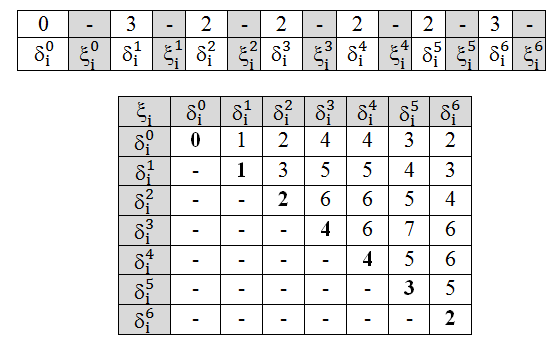
\includegraphics[width=0.45\textwidth]{algo_example.png}
\caption{Algorithm Example.}
\label{fig:algo_example}
\end{center}
\vspace{-10pt}
\end{figure}
Let $N_i=6$ and $Q_i=12$ for the following basic block structure with WCET and preemption costs shown in Figure~\ref{fig:algo_example}.  The algorithm computes and stores the cumulative non-preemptive execution costs for starting and ending basic block pairs in a matrix denoted $N_p$.  Using this information, the combined WCET and CRPD costs for each basic block pair is computed and stored in a matrix denoted $q_{i}$.  These matrices are shown in Figure~\ref{fig:algo_example_2}.  The shaded cells in the $q_{i}$ matrix represent cases where the combined WCET and CRPD costs for these basic block pairs exceed the maximum allowable non-preemptive region parameter $Q_i$.  During execution of the algorithm, the minimum combined WCET + CRPD costs are computed for each basic block pair and stored in a matrix denoted $B_{i}$.  The $B_{i}$ matrix stores the non-preemptive execution cost above the diagonal and the preemptive execution cost below the diagonal.  Basic block pairs with preemptive costs that are less than or equal to $Q_i$ are candidates for selection.  When a lower cost is determined for a given basic block pair, the predecessor preemption point is updated in the $\rho_{prev}$ array which keeps track of the selected predecessor preemption point for each basic block forming a daisy chain containing the entire set of selected preemption points.  The final results are illustrated in Figure~\ref{fig:algo_example_3}.
\begin{figure}[h!]
\vspace{-10pt}
\begin{center}
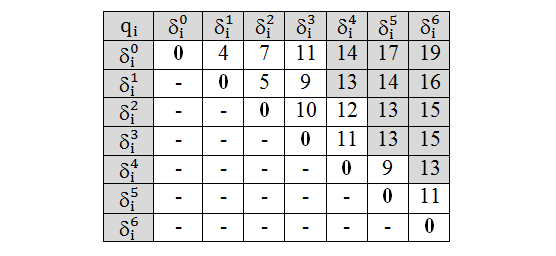
\includegraphics[width=0.45\textwidth]{algo_example_2.png}
\caption{Combined WCET and CPRD Costs.}
\label{fig:algo_example_2}
\end{center}
\vspace{-10pt}
\end{figure}
\begin{figure}[h!]
\vspace{-10pt}
\begin{center}
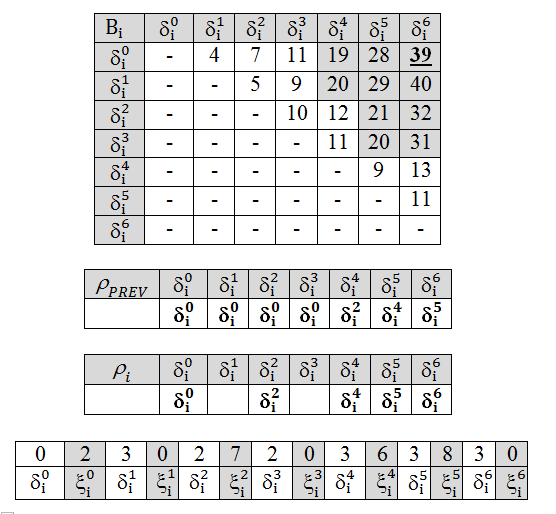
\includegraphics[width=0.45\textwidth]{algo_example_3.png}
\caption{Algorithm Results.}
\label{fig:algo_example_3}
\end{center}
\vspace{-10pt}
\end{figure}
